
\section{Methodology}

\subsection{Julia Language}
Julia is relatively new dynamic programming language, 
reaching stable release of 1.0 in August 2018 \citep{JuliaV1}.
It is a performant language with an empahsis
on productivity. Even though Julia has focus on scientific 
computing it considered as a general purpose programming
language. Some of its features include
multiple dispatch, just-in-time compilation and built-in
matrix data types \citep{Julia}.

Julia fits well for building an artificial market.
Artificial markets can be seen as a set of objects
and interactions in between, as described \citet{Ben12},
and in such models object-oriented programming (OOP)
is required. Even though Julia is more functional, OOP
architecture can be constructed with use of Julia's 
structs and type annotated functions. Also, the 
speed of code execution, support for matrix operations 
and good productivity makes it viable language for 
prototyping simulation systems. 


\begin{lstlisting}
#= This is a code sample for the Julia language
(adapted from http://julialang.org) =#
struct Market
    
\end{lstlisting}


\subsection{Generic Structure of the Model}
% Describe the generic structure (Type hierarchy, layers etc.)
% Kind of the static side of the simulation
The ASM model has three layers: abstraction layer, concrete 
layer and simulation layer. The fist layer contains the 
generic parts of the framework that are independent on the concrete
type of the elements. For example, this layer defines how 
to get traders' positions, how the trades are formed from
orders and all the abstract types. The main purpose of this layer
is to separate generic and obvious functionality from blocks of code
that has more degrees of freedom.

The second layer, the concrete layer, defines the actual types and
functionalities that are require less clear and more heuristic
approach than the abstract layer. This layer also include significant
portion of choices to make choices to make. Some of the components
on this layer include the zero intelligent investor and its
functions that defines its behaviour, the continuous double auction
market, its price mechanics and the interaction between investors
and markets.

The third layer, simulation layer, manages the simulation as a whole.
This layer defines ecosystem where the simulation takes place including
the initiation of the components, interating over the time periods, asking
each investor to make their decisions et cetera. Also the number of investors,
initial conditions such as amount of assets the investors own and how the 
simulation results are saved are defined here. This layer mostly calls
the functionalities created in the lower layers.



\subsection{Simulation Process}
% Describe how it works, how the dynamics flow etc.
In functional sense, the model consists of three main components:
the main level code, traders and markets. The main level code 
orchestrates the flow of the simulation while traders and markets
handle the pieces of functionalities associated with them. The process
is generalized in ~\ref{fig:sim_proc}. The beginning and the end of the 
simulation are shown in orange in the figure. Yellow boxes represent
the actions that belongs to the concrete layers and all the actions that
are in the main are part of the simulation layer. The remaining belong
generally to the abstract layer.


\begin{figure}
    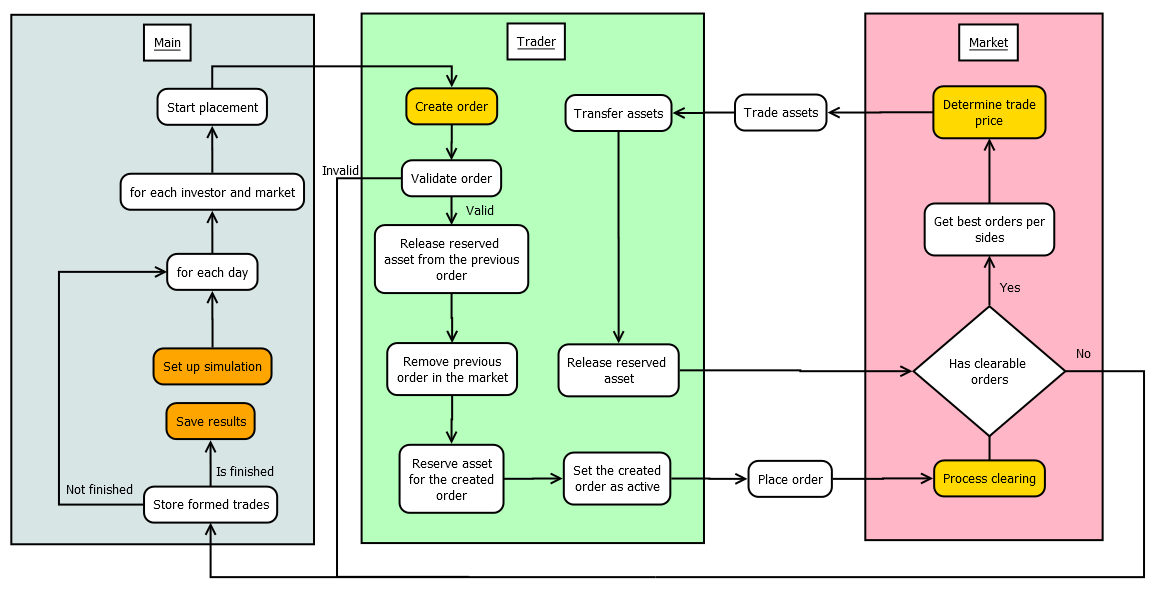
\includegraphics[width=\linewidth]{diagrams/placement_clearing_process.png}
    \caption{Simulation process}
    \label{fig:sim_proc}
\end{figure}

The simulation begins with setting up the parameters such as number of
trading days and initializing the traders, their assets and the markets.
Then each trading session is iterated in which each trader can create order 
an order to each market. After the order creation the order is validated.
The traders have also an option not to create an order. If the order was
valid, the previous order to the market is cancelled and the needed 
asset is reserved for the order in case it executes. The asset
reservation is to prevent traders going over their budgets if they
have allocated the same asset in other markets. Next the order is
placed to the market and the clearing process begins in case of 
continuous double auction market. If there are any clearable orders,
they are traded with a price defined by the market type. When
all clearable orders are cleared, the process returns to the
main block and either next trading session is started or the next
trader gets chance to make orders. In this section, the process how the
zero intelligent traders conduct their decisions and how the 
market price formation and clearing works is discussed with more detail.
There are some interesting characteristics in the asset dynamics of this
artificial market and these are also discussed.

\subsubsection{Trader Behaviour}
% How the investors make decisions actually

As mentioned, the traders of this model are zero intelligent
traders.

The placement decision requires three things to be defined: 
side of the order, quantity of the order and price of the order. 
These decisions are isolated as much as possible but there 
are some unavoidable dependencies in between. In order to
define the limits for the quantity, one must know 

The side of the order is determined picking randomly
between nothing, bid order and ask order. Nothing
represents that the trader did not want to create 
an order.

The quantity of the order is initially defined as the
amount of asset to allocate or commit for the order. 
In case of bid order, this amount of asset is the one that acts
like a currency in the market. For ask orders, this 
is the amount of traded asset, for example stocks. In 
case of bid order, this amount is converted to the 
amount of stocks when the price is decided. The quantity
of the asset to allocate is picked from a uniform distribution
in which the minimum is one and maximum is the total 
amount of the said asset the trader has unallocated in the
position. 

The price picked from a normal distribution in which the
mean price is the last market price and the standard
deviation is a constant parameter for the simulation.
The distribution is truncated in a way that the minimum
value is one and the maximum is the unallocated amount
in case of bid order and infinite in case of ask order.
This is due to buyer-seller asymmetricity which is discussed
in the handling of assets with more detail. The price
is rounded to nearest integer.



\subsubsection{Order Placement}
% How the orders are set to the markets, validated
% and how 

\subsubsection{Clearing Mechanics}
% How the market is cleared actually 


\subsubsection{Handling of Assets}
% Why use integers as units for assets

The model is constructed in a way that enables usage of multiple assets
and the assets are handled symmetrically. The former is achieved with
allowing multi-asset positions and it is the simulation layer's 
responsibility to decide the assets, markets and ask the investors
to create orders on them.

The asset symmetricity means that there is no universal or central currency 
and the currencies are handled as any other asset. In theoretical sense, 
currencies are also just investment options and there is no inherent reason why other 
asset classes, such as stocks, could not operate as the definition 
of value. This feature caused the model to be somewhat complex but 
abstracted the structure in a way that it handles natively cross currency
markets or ecosystems where there exists markets between assets A and 
B and between B and C but not between A and C. 

Asset symmetricity is constructed via storing all the owned and reserved
assets in the same data structures, in dictionaries in this case. In addition
to the traded asset, the markets contains also the information about the asset
that the traded asset is traded with, which is most often some sort of currency. 

All quantities of assets are stored as integers to prevent wealth leakage
or creation because of the floating point arithmetics. Using integers also
conveniently act as the tick size for all the markets. This also has the side effect
of that also all the prices must be represented as integers as one piece
of traded asset must equal exact quantity of the asset used as a currency
in the market. Furthermore, this creates deficency in the market if the quantities
of owned assets are small and also a phenomenon of asymmetricity between buyers and sellers
araises. The price set by an asker can be virtually anything: they can set
arbitrary positive price for their order as the only limitation is the amount
of traded asset they can commit to the order which is independent on the price. 
Every unit of increase in order price means more profit for the seller
in case the order is executed. On the otherhand, because of the 
lower limit of one in price the bidder does not have the same freedom.
The maximum price the bidder can set equals to the quantity of the asset
that behaves as currency in the market but the minimum price is one. This is
illustrated in the figure ~\ref{fig:buy_sell_asym} in which the all possible
combinations of quantities and prices are shown. The buyer owns
ten units of currency and the seller owns ten units of traded stock in
this example. The colored areas represent where the possible combinations
lie.
% About how this integer acts like tick in the market (1 unit of price = 1 tick)
 % And what this causes etc.
 % Price can be anything for seller but for buyer, there are boundaries

 \begin{figure}
    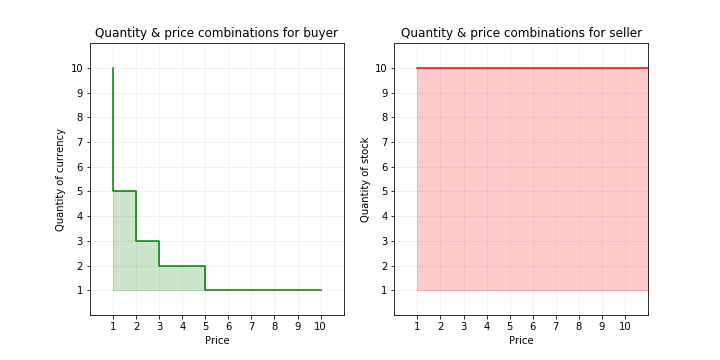
\includegraphics[width=\linewidth]{plots/buyer_seller_asymmetricity.png}
    \caption{Illustration of buyer-seller asymmetricity}
    \label{fig:buy_sell_asym}
\end{figure}